\documentclass[border=0.8ex,svgnames,tikz]{standalone}
\usepackage{amsmath,mathtools}
\usepackage{fontspec}
\setmainfont{Source Serif 4}
\setsansfont{Source Sans 3}
\setmonofont{Source Code Pro}
\begin{document}
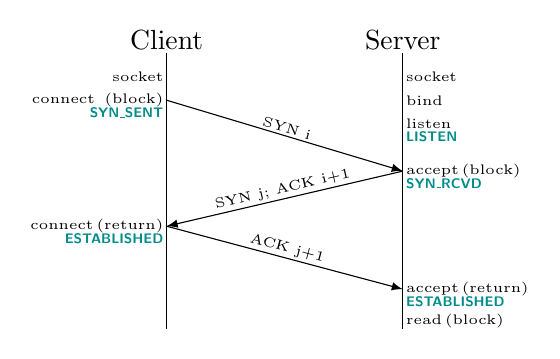
\begin{tikzpicture}[
  every label/.style={font=\tiny},
  every node/.style={inner sep=1pt,above,sloped,font=\tiny},
  status node/.append style={text=DarkCyan,font=\tiny\sf\bfseries},
  ]
  \path[draw] (0,0) coordinate(client-begin)
    node[above,font=\normalsize]{Client} -- (0,-3.5);
  \path[draw] (client-begin)
    ++(0,-0.3) coordinate[label=left:{socket}](client-socket)
    ++(0,-0.3) coordinate[label=left:{connect\, (block)}](client-connect-block)
    ++(0,-1.6) coordinate[label=left:{connect\,(return)}](client-connect-return);
  \path (client-connect-block)  ++(0,-0.16) node[left,status node]{SYN\_SENT}
        (client-connect-return) ++(0,-0.16) node[left,status node]{ESTABLISHED};

  \path[draw] (3,0) coordinate(server-begin)
    node[above,font=\normalsize]{Server} -- (3,-3.5);
  \path[draw] (server-begin)
    ++(0,-0.3) coordinate[label=right:{socket}](server-socket)
    ++(0,-0.3) coordinate[label=right:{bind}](server-bind)
    ++(0,-0.3) coordinate[label=right:{listen}](server-listen)
    ++(0,-0.6) coordinate[label=right:{accept\,(block)}](server-accept-block)
    ++(0,-1.5) coordinate[label=right:{accept\,(return)}](server-accept-return)
    ++(0,-0.4) coordinate[label=right:{read\,(block)}](server-read-block);
  \path (server-listen)        ++(0,-0.16) node[right,status node]{LISTEN}
        (server-accept-block)  ++(0,-0.16) node[right,status node]{SYN\_RCVD}
        (server-accept-return) ++(0,-0.16) node[right,status node]{ESTABLISHED};

  \path[draw] (client-connect-block)  edge[-latex] node{SYN i}
                (server-accept-block)
              (server-accept-block)   edge[-latex] node{SYN j; ACK i+1} (client-connect-return)
              (client-connect-return) edge[-latex] node{ACK j+1}        (server-accept-return);
\end{tikzpicture}
\end{document}
